\begin{frame}
    \frametitle{Działanie}
    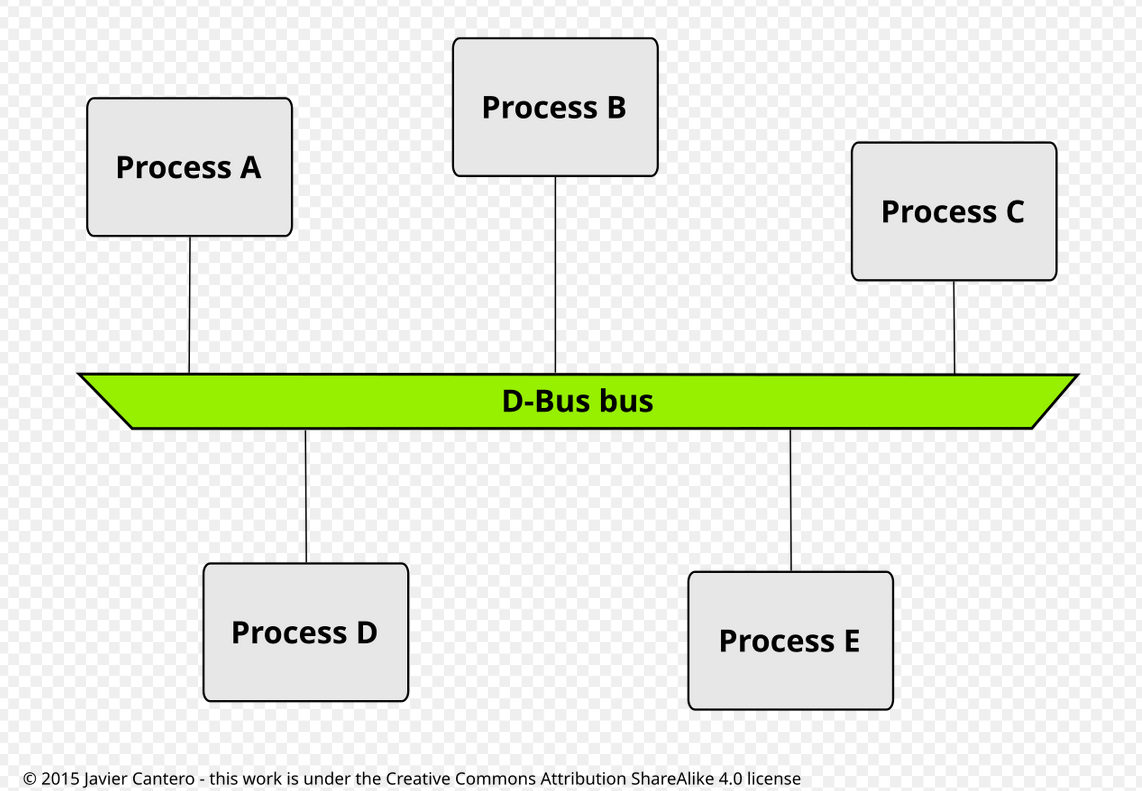
\includegraphics[width=\textwidth,height=\textheight,keepaspectratio]{dbus.png}
\end{frame}



\begin{frame}
    \frametitle{D-Bus bus}
    Demon do którego łączą się aplikacje. Przekierowuje
    wiadomości od aplikacji do innych aplikacji. Podział na 
    system bus i session bus.
\end{frame}

%\begin{frame}
%    \frametitle{libdbus}
%    Niskopoziomowa biblioteka pozwalająca aplikacjom na wymianę 
%    wiadomości.
%\end{frame}

\begin{frame}
    \frametitle{Session bus}
    Z poziomu użytkownika, osobna instancja dla każdego.
    \begin{itemize}
        \item DE KDE, GNOME 
        \item Aplikacje, Spotify, Firefox
        \item PulseAudio
    \end{itemize}
\end{frame}

\begin{frame}
    \frametitle{System bus}
    Z poziomu systemu operacyjnego. Pojedyncza instancja
    dla każdego użytkownika.
    \begin{itemize}
        \item Sieci, NetworkManager
        \item Urządzenia, UDisks
        \item Uprawnienia, PolicyKit
    \end{itemize}
\end{frame}

\begin{frame}
    \frametitle{Połączenie serwisu}
    Następuje przy połączeniu do demona.
    Serwis ma przyznawaną nazwę.
    \begin{itemize}
        \item Unikalna: :1-37, :1-42
        \item Well-known name: org.Cinammon, org.mpris.MediaPlayer2.spotify
    \end{itemize}
    Demon mapuje well-known name na nazwę unikalną.\linebreak
    Coś jak dns.
\end{frame}


\begin{frame}
    \frametitle{Interfejsy}
    Zbiór metod, sygnałów oraz właściwości (properties).
    Implementowane przez obiekty. 
    Coś jak abstract class.
    \begin{itemize}
        \item org.mpris.MediaPlayer2.Player
        \item org.freedesktop.Notifications
        \item org.freedesktop.NetworkManager
        \item org.freedesktop.UDisks2.Drive
    \end{itemize}
\end{frame}

\begin{frame}
    \frametitle{Obiekt}
    \begin{itemize}
        \item Wymaga określenia bus name 
        \item Ścieżka do obiektu jako nazwa:
        \begin{itemize}
            \item /org/mpris/MediaPlayer2 
            \item /org/freedesktop/Notifications
            \item /org/freedesktop/NetworkManager
            \item /org/freedesktop/UDisks2/drives/KINGSTON123afmaolk1
        \end{itemize}
        \item Implementuje interfejs lub interfejsy.
    \end{itemize}
\end{frame}



\begin{frame}
    \frametitle{Metody}
    Synchroniczne. Obiekt implementuje metodę którą
    klient może wywołać z argumentami. Może zwracać
    z powrotem wartość.
\end{frame}

\begin{frame}
    \frametitle{Sygnały}
    Asynchroniczne. Obiekt emituje sygnał.
    Klient nasłuchuje sygnałów i implementuje handler.
\end{frame}


\begin{frame}
    \frametitle{Interfejsy standardowe}
    Interfejsy zapewniające definicje metod, 
    przydatne przy implementacji serwisów.
    \begin{itemize}
        \item \href{https://dbus.freedesktop.org/doc/dbus-java/api/org/freedesktop/DBus.Peer.html}{org.freedesktop.DBus.Peer} - metody Ping i GetMachineId \pause
        \item \href{https://dbus.freedesktop.org/doc/dbus-java/api/org/freedesktop/DBus.Introspectable.html}{org.freedesktop.DBus.Introspectable} - reprezentacja obiektu w XML \pause
        \item \href{https://dbus.freedesktop.org/doc/dbus-java/api/org/freedesktop/DBus.Properties.html}{org.freedesktop.DBus.Properties} - manipulacja właściwościami, odczyt wartości \pause
        \item \href{URL}{org.freedesktop.DBus.ObjectManager} - zarządzanie obiektami udostępnianymi przez serwis
    \end{itemize}
\end{frame}


\begin{frame}
    \frametitle{Przykład}
    \begin{columns}
    \begin{column}{0.5\textwidth}
        \begin{center}
            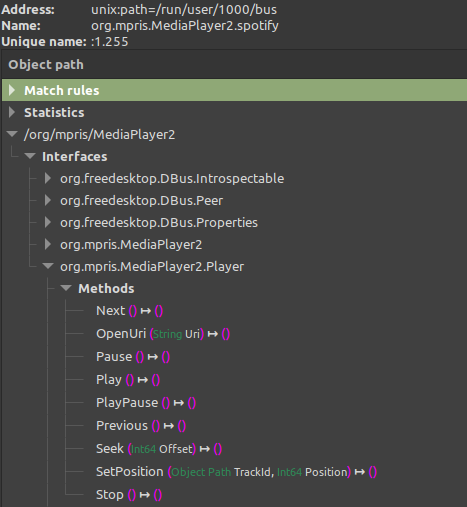
\includegraphics[width=\textwidth,height=\textheight,keepaspectratio]{service1.png}
        \end{center}
    \end{column}
    \begin{column}{0.5\textwidth}
        \begin{center}
            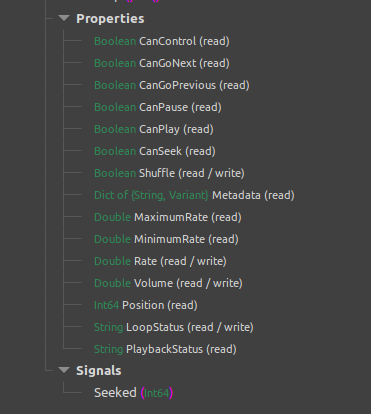
\includegraphics[width=\textwidth,height=\textheight, keepaspectratio]{example2.png}        
        \end{center}
    \end{column}
\end{columns}
\end{frame}



\begin{frame}[fragile]
    \frametitle{Proxy}
    Obiekt tworzony przez klienta jako reprezentacja
    zdalnego obiektu innego procesu. Niskopoziomowo tworzy
    wiadomość do serwisu z requestowanym wykonaniem metod i zwraca
    odpowiedź.

    \begin{flushleft}
        \begin{lstlisting}
bus = SessionBus()
proxy = bus.get(SERVICE_NAME, SERVICE_OBJECT)
method_res = proxy[INTERFACE_NAME].Method(a1, a2)

proxy.SomeSignal().connect(SIGNAL_HANDLER)
loop.run()
        \end{lstlisting}      
    \end{flushleft}

\end{frame}

\begin{frame}
    \frametitle{Wiadomości niskopoziomowo}
    Dzielą się na 4 typy:
    \begin{itemize}
        \item Wiadomości wywołujące metody
        \item Wiadomości zwracające return value metody
        \item Błędy zwracające wyjątki spowodowane 
        wywołaniem metody. Zła walidacja typu, 
        brak autoryzacji, brak serwisu, obiektu itp.
        \item Asynchroniczne sygnały
    \end{itemize}
\end{frame}

\begin{frame}
    \frametitle{Wiadomości niskopoziomowo cd.}
    Coś takiego:
    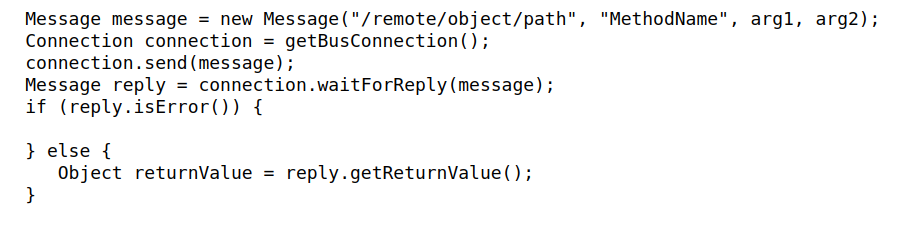
\includegraphics[width=\textwidth]{low_level.png}
\end{frame}

\begin{frame}
    \frametitle{System typów}
    \href{https://dbus.freedesktop.org/doc/dbus-specification.html}{Parę przykładów:}
    \begin{itemize}
        \item aai - tablica tablic intów \pause
        \item a(ss) - array structów z dwoma stringami \pause
        \item a\{sd\} - mapa klucz-string value-double \pause
        \item v - variant, dynamiczny typ opakowany w klasę Variant \pause
        \item a\{sv\} - mapa z wartościami o różnych typach \pause
        \item Ale tak naprawdę wszystko jest variantem (enkapsulacja)
    \end{itemize}
\end{frame}





% https://dbus.freedesktop.org/doc/dbus-api-design.html